\chapter{Mathematical basics}
This appendix covers the most important mathematical basics, that were used in this thesis. More information can be found in the books \cite{Durandi:2009, Schwarz:2011, Rudolf:2014, Taschner:2014, Taschner:2015, Kugi:2021}.

%% Trigonometry %%
\section{Trigonometry} \label{sec:trigonometry}

\begin{center}
	\begin{equation} \label{eq:addition_theorem_cos}
		\cos \left(x \pm y\right) = \cos x \, \cos y \mp \sin x \, \sin y
	\end{equation}
\end{center}

\begin{center}
	\begin{equation} \label{eq:addition_theorem_sin}
		\sin \left(x \pm y\right) = \sin x \, \cos y \pm \cos x \, \sin y
	\end{equation}
\end{center}

\begin{center}
	\begin{equation} \label{eq:reduction_formula}
		\sin \left(90^\circ - x \right) = \cos x
	\end{equation}
\end{center}

\begin{center}
	\begin{equation} \label{eq:sin_squared}
		\sin^2 \frac{\beta}{2} = \frac{1 - \cos \beta}{2}
	\end{equation}
\end{center}

\begin{center}
	\begin{equation} \label{eq:cos_squared}
		\cos^2 \frac{\beta}{2} = \frac{1 + \cos \beta}{2}
	\end{equation}
\end{center}

%% Integral of the Gaussian bell function %%

\section{Integral of the Gaussian bell curve} \label{sec:gauss_general}
In this thesis, the shifted Gaussian bell function, shown in figure \ref{fig:tikz_gauss_curve_general}, is used to model the solar energy curve (see subsection \ref{sec:solar_energy_curve}). Therefore the mathematical approach of calculating the area of the Gaussian bell function -- enclosed by the curve and the x-axis -- will be explained.
\begin{figure}[h!]
	\centering
	
\tikzset{every picture/.style={line width=0.75pt}} %set default line width to 0.75pt        

\begin{tikzpicture}[x=0.75pt,y=0.75pt,yscale=-1,xscale=1]
%uncomment if require: \path (0,300); %set diagram left start at 0, and has height of 300

%Image [id:dp36698085633645405] 
\draw (328.75,179) node  {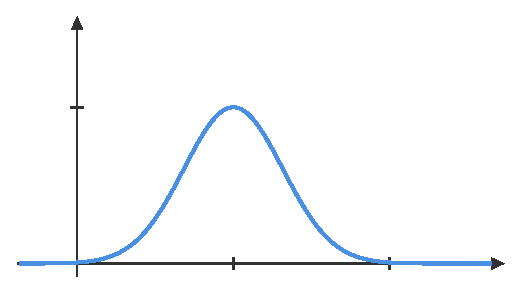
\includegraphics[width=233.63pt,height=124.5pt]{images/image_shifted_gauss_curve}};
%Straight Lines [id:da37857254246955074] 
\draw [color={rgb, 255:red, 155; green, 155; blue, 155 }  ,draw opacity=1 ] [dash pattern={on 4.5pt off 4.5pt}]  (222,153.7) -- (303.4,153.7) ;
%Straight Lines [id:da32947142925776296] 
\draw [color={rgb, 255:red, 155; green, 155; blue, 155 }  ,draw opacity=1 ] [dash pattern={on 4.5pt off 4.5pt}]  (311.4,243) -- (311.4,155.7) ;
%Shape: Circle [id:dp5744124003855682] 
\draw  [fill={rgb, 255:red, 255; green, 255; blue, 255 }  ,fill opacity=1 ] (309.4,153.7) .. controls (309.4,152.6) and (310.3,151.7) .. (311.4,151.7) .. controls (312.5,151.7) and (313.4,152.6) .. (313.4,153.7) .. controls (313.4,154.8) and (312.5,155.7) .. (311.4,155.7) .. controls (310.3,155.7) and (309.4,154.8) .. (309.4,153.7) -- cycle ;

% Text Node
\draw (202.5,76.9) node [anchor=north west][inner sep=0.75pt]  [font=\footnotesize]  {$f( x)$};
% Text Node
\draw (488,248.4) node [anchor=north west][inner sep=0.75pt]  [font=\footnotesize]  {$x$};
% Text Node
\draw (305,262.9) node [anchor=north west][inner sep=0.75pt]  [font=\footnotesize]  {$x_{0}$};
% Text Node
\draw (397.5,259.4) node [anchor=north west][inner sep=0.75pt]  [font=\footnotesize]  {$2x_{0}$};
% Text Node
\draw (197,256.4) node [anchor=north west][inner sep=0.75pt]  [font=\footnotesize]  {$0$};
% Text Node
\draw (191,147.4) node [anchor=north west][inner sep=0.75pt]  [font=\footnotesize]  {$C$};


\end{tikzpicture}


	\caption{Shifted Gauss bell.}
	\label{fig:tikz_gauss_curve_general}
\end{figure}

In general the function of the Gaussian bell function can be written as shown in equation \ref{eq:gauss_curve}, with its corresponding indefinite Integral shown in equation \ref{eq:integral_gauss}.
\begin{center}
	\begin{equation} \label{eq:gauss_curve}
		f\left(x\right) = C \, \exp\left(-\frac{(x - x_0)^2}{a}\right)
	\end{equation}
\end{center}
\begin{center}
	\begin{equation} \label{eq:integral_gauss}
		F\left(x\right) = C \int\limits_{-\infty}^{\infty} \exp\left(-\frac{(x - x_0)^2}{a}\right)\,\mathrm{d}x
	\end{equation}
\end{center}
Since the integral in equation \ref{eq:integral_gauss} cannot be solved, an approach is used in which the integral is squared. How this works is presented in the following steps.
\begin{center}
	\begin{equation} \label{eq:integral_gauss_partly_solved}
		\begin{aligned}
		F\left(x\right)^2 &= C^2 \left( \, \int\limits_{-\infty}^{\infty} \exp\left(-\frac{(x - x_0)^2}{a}\right)\,\mathrm{d}x\right)^2 \\
		&= C^2 \int\limits_{-\infty}^{\infty} \exp\left(-\frac{(u - u_0)^2}{a}\right)\,\mathrm{d}u \int\limits_{-\infty}^{\infty} \exp\left(-\frac{(v - v_0)^2}{a}\right)\,\mathrm{d}v \\ 
		&= C^2 \int\limits_{-\infty}^{\infty} \int\limits_{-\infty}^{\infty} \exp\left(-\frac{(u - u_0)^2}{a}\right) \, \exp\left(-\frac{(v - v_0)^2}{a}\right) \,\mathrm{d}u \cdot \mathrm{d}v \\
		&= C^2 \int\limits_{-\infty}^{\infty} \int\limits_{-\infty}^{\infty} \exp\left(-\frac{(u - u_0)^2 + (v - v_0)^2}{a}\right) \,\mathrm{d}u \cdot \mathrm{d}v
		\end{aligned}
	\end{equation}
\end{center}
If now $x = u - u_0$ and $y = v - v_0$ are substituted in the last step of equation \ref{eq:integral_gauss_partly_solved}, the integrals can be written as presented on the left side of equation \ref{eq:integral_gauss_not_shifted}. Due to the substitutions, the equations \ref{eq:diff} to \ref{eq:lim_y} have to be considered. 
\begin{center}
	\begin{equation} \label{eq:diff}
		\mathrm{d}x = \mathrm{d}u \text{, } \mathrm{d}y = \mathrm{d}v
	\end{equation}
\end{center}
\begin{center}
	\begin{equation} \label{eq:lim_x}
		\lim\limits_{u \to \infty} x = \infty \text{, } \lim\limits_{u \to -\infty} x = -\infty
	\end{equation}
\end{center}
\begin{center}
	\begin{equation} \label{eq:lim_y}
		\lim\limits_{v \to \infty} y = \infty \text{, } \lim\limits_{v \to -\infty} y = -\infty
	\end{equation}
\end{center}
Transforming the integrals on the left side of equation \ref{eq:integral_gauss_not_shifted} into polar coordinates, by using the expressions from equation \ref{eq:polar}, the integrals on the right side of equation \ref{eq:integral_gauss_not_shifted} follows.
\begin{center}
	\begin{equation} \label{eq:polar}
		x^2 + y^2 = r^2 \text{, } \mathrm{d}x \, \mathrm{d}y = r \, \mathrm{d}r \,\mathrm{d}\phi
	\end{equation}
\end{center}
\begin{center}
	\begin{equation} \label{eq:integral_gauss_not_shifted}
		\begin{aligned}
		F\left(x\right)^2 &= C^2 \int\limits_{-\infty}^{\infty} \int\limits_{-\infty}^{\infty} \exp\left(-\frac{x^2 + y^2}{a}\right) \,\mathrm{d}x \cdot \mathrm{d}y \\
		&= C^2 \int\limits_{0}^{2\pi} \int\limits_{0}^{\infty} \exp\left(-\frac{r^2}{a}\right) \, r \,\mathrm{d}r \cdot \mathrm{d}\phi
		\end{aligned}
	\end{equation}
\end{center}
With a final substitution of $w = -\frac{r^2}{a}$, form which the equations \ref{eq:diff_r} to \ref{eq:lim_r} derive, the integrals can be solved as shown in equation \ref{eq:integral_gauss_solved}.
\begin{center}
	\begin{equation} \label{eq:diff_r}
		r\,\mathrm{d}r = -\frac{a}{2} \, \mathrm{d}u
	\end{equation}
\end{center}
\begin{center}
	\begin{equation} \label{eq:lim_r}
		\lim\limits_{r \to \infty} w = -\infty \text{, } \lim\limits_{r \to 0} w = 0
	\end{equation}
\end{center}
\begin{center}
	\begin{equation} \label{eq:integral_gauss_solved}
		\begin{split}
		F\left(x\right)^2 = -\frac{a \, C^2}{2}\int\limits_{0}^{2\pi} \underbrace{\int\limits_{0}^{-\infty} \mathrm{e}^w \,\mathrm{d}w}_{-1} \cdot \mathrm{d}\phi = \frac{a \, C^2}{2}\int\limits_{0}^{2\pi} 1 \, \mathrm{d}\phi = a \, C^2 \, \pi
		\end{split}
	\end{equation}
\end{center}
Therefore the result of the indefinite integral of the Gaussian bell function must be:
\begin{center}
	\begin{equation} \label{eq:lim_r}
		F(x) = C \sqrt{a \, \pi} \text{.}
	\end{equation}
\end{center}
It is positive because the area enclosed by the curve and the x-axis cannot be negative. 

%% Newton method %%

\section{Newton-Raphson method} \label{sec:newton_raphson_method}
The zero crossing $x = x_R$ of a function $f\left( x \right) : \mathbb{R} \to \mathbb{R}$, for which $f\left( x_R \right) = 0$ aplies, can be approximated with the Newton-Raphson method as shown in equation \ref{eq:x_iteration}.
\begin{center}
	\begin{equation} \label{eq:x_iteration}
		\begin{gathered}
			x_1 = x_0 - \frac{f\left( x_0 \right)}{f'\left( x_0 \right)} \\
			x_2 = x_1 - \frac{f\left( x_1 \right)}{f'\left( x_1 \right)} \\
			\vdots \\
			x_{n + 1} = x_n - \frac{f\left( x_n \right)}{f'\left( x_n \right)}
		\end{gathered}
	\end{equation}
\end{center}
This algorithm can be derived with figure \ref{fig:tikz_newton_method}, whereby the requirement must be met that the function $f\left( x \right)$ must be continuously differentiable for the required number of iteration steps $n + 1$ with $n \in \mathbb{N}$.
\begin{figure}[h!]
	\centering
	
\tikzset{every picture/.style={line width=0.75pt}} %set default line width to 0.75pt        

\begin{tikzpicture}[x=0.75pt,y=0.75pt,yscale=-1,xscale=1]
%uncomment if require: \path (0,432); %set diagram left start at 0, and has height of 432

%Image [id:dp6404601341090801] 
\draw (359.5,218.99) node  {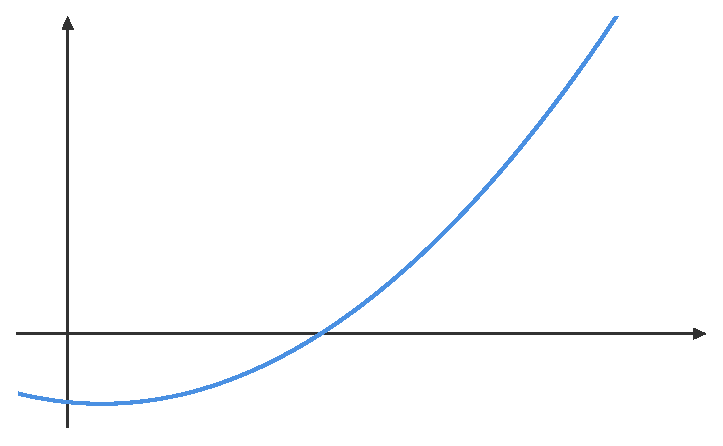
\includegraphics[width=330.75pt,height=197.25pt]{images/image_newton_method}};
%Straight Lines [id:da6424929768444043] 
\draw [color={rgb, 255:red, 155; green, 155; blue, 155 }  ,draw opacity=1 ][line width=0.75]  [dash pattern={on 4.5pt off 4.5pt}]  (510.1,106.5) -- (510.1,284.5) ;
%Straight Lines [id:da8758554517093697] 
\draw [color={rgb, 255:red, 155; green, 155; blue, 155 }  ,draw opacity=1 ]   (510.1,105.5) -- (382,289.33) ;
%Straight Lines [id:da8632115968328404] 
\draw [color={rgb, 255:red, 155; green, 155; blue, 155 }  ,draw opacity=1 ][line width=0.75]  [dash pattern={on 4.5pt off 4.5pt}]  (382,262.5) -- (382,285.33) ;
%Straight Lines [id:da10976638691733442] 
\draw [color={rgb, 255:red, 155; green, 155; blue, 155 }  ,draw opacity=1 ]   (340.5,289.5) -- (382,253.2) ;
%Straight Lines [id:da28590987584360095] 
\draw    (510.1,289.5) -- (510.1,293.2) ;
%Straight Lines [id:da06729921605109834] 
\draw    (510.1,286) -- (510.1,290) ;
%Straight Lines [id:da18775137309121925] 
\draw [color={rgb, 255:red, 155; green, 155; blue, 155 }  ,draw opacity=1 ]   (518.35,93.95) -- (510.1,105.5) ;
%Shape: Circle [id:dp7916165248356848] 
\draw  [fill={rgb, 255:red, 255; green, 255; blue, 255 }  ,fill opacity=1 ] (508.1,105.5) .. controls (508.1,104.4) and (509,103.5) .. (510.1,103.5) .. controls (511.2,103.5) and (512.1,104.4) .. (512.1,105.5) .. controls (512.1,106.6) and (511.2,107.5) .. (510.1,107.5) .. controls (509,107.5) and (508.1,106.6) .. (508.1,105.5) -- cycle ;
%Straight Lines [id:da1316603229735085] 
\draw    (382,289.5) -- (382,293.2) ;
%Straight Lines [id:da9560432424659024] 
\draw    (340.5,289.5) -- (340.5,293.2) ;
%Straight Lines [id:da2626747830873235] 
\draw    (382,286) -- (382,290) ;
%Straight Lines [id:da9507317011882577] 
\draw    (340.5,285.5) -- (340.5,289.5) ;
%Straight Lines [id:da6325259503800027] 
\draw [color={rgb, 255:red, 155; green, 155; blue, 155 }  ,draw opacity=1 ]   (382,253.2) -- (423.5,216.9) ;
%Shape: Circle [id:dp23034405156952054] 
\draw  [fill={rgb, 255:red, 255; green, 255; blue, 255 }  ,fill opacity=1 ] (380,253.2) .. controls (380,252.1) and (380.9,251.2) .. (382,251.2) .. controls (383.1,251.2) and (384,252.1) .. (384,253.2) .. controls (384,254.3) and (383.1,255.2) .. (382,255.2) .. controls (380.9,255.2) and (380,254.3) .. (380,253.2) -- cycle ;
%Straight Lines [id:da641645989007537] 
\draw [color={rgb, 255:red, 155; green, 155; blue, 155 }  ,draw opacity=1 ]   (526.6,82.4) -- (518.35,93.95) ;

% Text Node
\draw (162,68.4) node [anchor=north west][inner sep=0.75pt]  [font=\footnotesize]  {$f( x)$};
% Text Node
\draw (503.5,298.4) node [anchor=north west][inner sep=0.75pt]  [font=\footnotesize]  {$x_{0}$};
% Text Node
\draw (375.5,298.4) node [anchor=north west][inner sep=0.75pt]  [font=\footnotesize]  {$x_{1}$};
% Text Node
\draw (585,285.4) node [anchor=north west][inner sep=0.75pt]  [font=\footnotesize]  {$x$};
% Text Node
\draw (334,298.4) node [anchor=north west][inner sep=0.75pt]  [font=\footnotesize]  {$x_{2}$};
% Text Node
\draw (524,106) node [anchor=north west][inner sep=0.75pt]  [font=\footnotesize,color={rgb, 255:red, 155; green, 155; blue, 155 }  ,opacity=1 ] [align=left] {Curve tangent\\at point $\displaystyle x_{0}$.};
% Text Node
\draw (304,209) node [anchor=north west][inner sep=0.75pt]  [font=\footnotesize,color={rgb, 255:red, 155; green, 155; blue, 155 }  ,opacity=1 ] [align=left] {Curve tangent\\at point $\displaystyle x_{1}$.};


\end{tikzpicture}


	\caption{Newton-Raphson method to approximate the zero crossing of a function.}
	\label{fig:tikz_newton_method}
\end{figure}
The approximation of the zero crossing $x_R$ -- taking into account the just mentioned requirement -- can be determined with any specified precision $\left| x_{n + 1} - x_n \right| < \varepsilon$. In order for the algorithm to converge towards the zero crossing, the start value $x_0$ must be found accordingly.

Based on the previous findings, the elements of the vector of zero crossings $\mathrm{\mathbf{x}} = \mathrm{\mathbf{x}}_R$ of the vector of functions $\mathrm{\mathbf{f}} \left( \mathrm{\mathbf{x}} \right) : \mathbb{R}^m \to \mathbb{R}^m$ with $m \in \mathbb{N}$, for which $\mathrm{\mathbf{f}}\left( \mathrm{\mathbf{x}}_R \right) = \mathbf{0}$ applies, can be approximated as shown below.
\begin{center}
	\begin{equation} \label{eq:vect_x_approx}
		\mathrm{\mathbf{x}}_{R, n + 1} = \mathrm{\mathbf{x}}_{R,n} 	- \mathrm{\mathbf{J}}^{-1}\left( \mathrm{\mathbf{x}}_{R,n} \right) \, \mathrm{\mathbf{f}}\left( \mathrm{\mathbf{x}}_{R,n} \right) 
	\end{equation}
\end{center}
The Jacobian matrix $\mathrm{\mathbf{J}}$ contains all partial derivatives of the function vector with respect to the vector of the zero crossings.
\begin{center}
	\begin{equation} \label{eq:jacobian}
		\mathrm{\mathbf{J}} = \left. \dfrac{\partial \mathrm{\mathbf{f}}\left(\mathrm{\mathbf{x}}\right)}{\partial \mathrm{\mathbf{x}}} \right|_{\mathrm{\mathbf{x}} = \mathrm{\mathbf{x}}_R} = 
 		\begin{pmatrix}
  			\dfrac{\partial}{\partial x_1} f_1\left( \mathrm{\mathbf{x}}_R \right) & \dfrac{\partial}{\partial x_2} f_1\left( \mathrm{\mathbf{x}}_R \right) & \cdots & \dfrac{\partial}{\partial x_m} f_1\left( \mathrm{\mathbf{x}}_R \right) \\
			\dfrac{\partial}{\partial x_1} f_2\left( \mathrm{\mathbf{x}}_R \right) & \dfrac{\partial}{\partial x_2} f_2\left( \mathrm{\mathbf{x}}_R \right) & \cdots & \dfrac{\partial}{\partial x_m} f_2\left( \mathrm{\mathbf{x}}_R \right) \\
			\vdots & \vdots & \ddots & \vdots \\
  			\dfrac{\partial}{\partial x_1} f_m\left( \mathrm{\mathbf{x}}_R \right) & \dfrac{\partial}{\partial x_2} f_m\left( \mathrm{\mathbf{x}}_R \right) & \cdots & \dfrac{\partial}{\partial x_m} f_m\left( \mathrm{\mathbf{x}}_R \right) 
 		\end{pmatrix}
 	\end{equation}
\end{center}
For completeness it shall be mentioned, that $ \mathrm{\mathbf{x}}_R = \big( x_1, \dotsc, x_m \big)^{\mathrm T } $ does not correspond to figure \ref{fig:tikz_newton_method}. The elements $x_1$ to $x_m$ of the vector $\mathrm{\mathbf{x}}_R$ are zero crossings of the functions contained by the vector $\mathrm{\mathbf{f}} \left( \mathrm{\mathbf{x}}_R \right) = \big( f_1\left( \mathrm{\mathbf{x}}_R \right), \dotsc, f_m\left( \mathrm{\mathbf{x}}_R \right) \big)^{\mathrm T } = \mathbf{0}$. Their $\left(n + 1\right)$\textsuperscript{th} approximation is $\mathrm{\mathbf{x}}_{R,n + 1} = \big( x_{1,n + 1}, \dotsc, x_{m,n + 1} \big)^{\mathrm T}$.







